\documentclass[12pt,a4paper,aspectratio=169]{beamer}
\usepackage[latin1]{inputenc}
\usepackage{textgreek}
\usepackage{graphicx,txfonts}
\usepackage{listings}
\usepackage{textcomp}

% some stylistic customizations...
\setbeamertemplate{navigation symbols}{}
\definecolor{my_lblue}{HTML}{2A8592}
\definecolor{my_yellow}{HTML}{85922A}
\definecolor{my_purple}{HTML}{922A85}
\definecolor{my_green}{HTML}{2A9236}
\definecolor{my_blue}{HTML}{382A92}
\definecolor{my_brown}{HTML}{92382A}
\definecolor{egym_orange}{rgb}{.93, .46, 0}
\usecolortheme[RGB={239,124,0}]{structure}
\setbeamertemplate{itemize items}{\textbullet}

\newcommand{\heart}{\ensuremath\varheartsuit}

\setbeamertemplate{frametitle}{
    \vspace{1.75em}
    \insertframetitle
}

\defbeamertemplate*{title page}{mydefault}[1][]
{
    \vskip.5em
    \includegraphics[width=6em]{egym}
    \vskip-5em

    \begin{center}
    \vfill
    \vskip3em
    {{\color{structure}\usebeamerfont{title}\inserttitle}\par
      \ifx\insertsubtitle
      \else%
        \vskip0.25em%
        {\usebeamerfont{subtitle}\usebeamercolor[fg]{subtitle}\insertsubtitle\par}%
      \fi }
    \vskip1em
    {    \usebeamerfont{author}\insertauthor\par    }
    \vskip0.5em
    {    \usebeamerfont{date}\insertdate\par    }
  \vfill
    \end{center}
}

\title{Distributed System Erlang Style}
\author{Robert Lemmen \textless robert.lemmen@egym.de\textgreater}
\date{\today}

\begin{document} {

\frame {
    \titlepage
}

\frame {
    \begin{center}
    \begin{tabular}{cl} 
    \begin{tabular}{c}
    \includegraphics[height=.75\textheight]{Erlang.jpg}
    \end{tabular}
    \begin{tabular}{l}
    \parbox{0.5\linewidth}{
    \textbf{Agner Krarup Erlang} \\ Born 1.1.1878 in L\o nborg, Denmark. Died
3.2.1929. \\ ~ \\ 1909: ``The Theory of Probabilities and Telephone Conversations''}
    \end{tabular}  \\
    \end{tabular}
    \end{center}
}

\frame {
    \begin{center}
    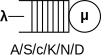
\includegraphics[scale=.5]{kendall1.pdf}
    \end{center}
}

\frame {
    \begin{center}
    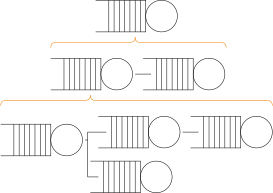
\includegraphics[scale=.4]{kendall2.pdf}
    \end{center}
}

\frame {
    \begin{center}
    \includegraphics[width=\textwidth]{../01-events.pdf}
    \end{center}
}

\frame {
    \begin{center}
    \includegraphics[width=\textwidth]{../01-histogram.pdf}
    \end{center}
}

\frame {
    \center\large\color{egym_orange} 1. Real world events are poisson
distributed over time, which is a pathological case
}

\begin{frame}[fragile] 
{\color{blue}https://github.com/robertlemmen/qsim/}
\begin{lstlisting}[language=Perl,basicstyle=\footnotesize]
sub random-events($basename, &random-func) {
    my $i = 0;
    my @hist;
    my $event-fh = open("{$basename}-events.data", :w);
    my $histogram-fh = open("{$basename}-hist.data", :w);
    while $i < samples-total {
        my $sample = &random-func();
        $i += $sample;
        if $i < event-window {
            $event-fh.say($i);
        }
        my $idx = round($sample/bin-size); 
        @hist[$idx]++;
    }
    for ^hist-width -> $idx {
        my $cv = @hist[$idx] // 0;
        if $idx > 0 {
            $histogram-fh.say("{$idx * bin-size} $cv");
        }
    }
    $event-fh.close;
    $histogram-fh.close;
}
\end{lstlisting}
\end{frame}

\begin{frame}[fragile]
\vspace{.5em}
\begin{lstlisting}[language=Perl,basicstyle=\footnotesize]
my $example = TestBed.new(producer-func => sub () { 
    return (random-poisson-distance(35), "m") });
my $q1 = Queue.new(id => "q1", size => 5);
my $p1 = Processor.new(id => "p1", capacity => 1, 
    proc-func => sub ($msg) { 
        return (random-poisson-distance(30), $message ~ '+') });

connect($example, $q1);
connect($q1, $p1);
connect($p1, $example);
\end{lstlisting}
\vspace{.5em}
    \includegraphics[width=\textwidth]{simple1.pdf}
\end{frame}

% XXX hyper code sample

\frame {
    \begin{center}
    \includegraphics[width=\textwidth]{../02-simple-queue.pdf}
    \end{center}
}

\frame {
    \begin{center}
    \includegraphics[width=\textwidth]{../02-simple-queue-2.pdf}
    \end{center}
}

\frame {
    \center\large\color{egym_orange} 2. Queues in a working system are almost
always very short
}

\frame {
    \begin{center}
    \includegraphics[width=\textwidth]{../02-simple-queue-2.pdf}
    \end{center}
}

\frame {
    \begin{center}
    \includegraphics[width=\textwidth]{../02-simple-queue-3.pdf}
    \end{center}
}

\frame {
    \center\large\color{egym_orange} 3. Perfect concurrency makes the outliers in
arrival or processing times statistical
}

\begin{frame}[fragile]
\vspace{1em}
\begin{lstlisting}[language=Perl,basicstyle=\footnotesize,deletekeywords={time}]
sub tb-producer() {
    my $interval = 100;
    if 2000 < $*current-time < 8000 {
        $interval = 35;
    }
    return (random-poisson-distance($interval), "");
}
\end{lstlisting}
\end{frame}

\frame {
    \begin{center}
    \includegraphics[width=\textwidth]{../03-ramp.pdf}
    \end{center}
}

\begin{frame}[fragile]
\vspace{1em}
\begin{lstlisting}[language=Perl,basicstyle=\footnotesize,deletekeywords={time}]
sub p2-processor($message) {
    return (random-poisson-distance(240 * 1.09 ** $*concurrency), 
        $message ~ '+');
}
\end{lstlisting}
\end{frame}

\frame {
    \begin{center}
    \includegraphics[width=\textwidth]{../05-hysteresis.pdf}
    \end{center}
}

\frame {
    \center\large\color{egym_orange} 4. Imperfect concurrency leads to
hysteresis 
}

\frame {
    \begin{center}
    \includegraphics[width=\textwidth]{../04-overload.pdf}
    \end{center}
}

\frame {
    \center\large\color{egym_orange} 5. Recovery from overload in a efficiently
sized system can take a long time
}

\frame {
    \begin{center}
    \includegraphics[width=\textwidth]{../06-baseline.pdf}
    \end{center}
}

\frame {
    \begin{center}
    \includegraphics[width=\textwidth]{../06-qlimit.pdf}
    \end{center}
}

\frame {
    \center\large\color{egym_orange} 6. Limiting queues is efficient in aiding
recovery, but is still relatively slow at clearing queues
}

\frame {
    \begin{center}
    \includegraphics[width=\textwidth]{../07-deadlines.pdf}
    \end{center}
}

% XXX processing time distribution

\frame {
    \center\large\color{egym_orange} 7. Deadlines are excellent at clearing
queues, but are hard to configure aggressively enough
}

\frame {
    \begin{center}
    \includegraphics[width=\textwidth]{../08-both.pdf}
    \end{center}
}

% XXX processing time distribution

\frame {
    \center\large\color{egym_orange} 8. The two methods to aid recovery
compliment each other well
}

% XXX unlimited concurrency breaks both

% XXX conclusions

\end{document}
